\documentclass{jarticle}
\pagestyle{empty}
\usepackage{graphicx}
\usepackage{booktabs}
\setlength{\topmargin}{-10.4mm}
\setlength{\headheight}{0mm}
\setlength{\headsep}{0mm}
\setlength{\textheight}{262mm}
\setlength{\textwidth}{180mm}
%\setlength{\topskip}{7mm}
\setlength{\evensidemargin}{-10.4mm} 
\setlength{\oddsidemargin}{-10.4mm} 
\setlength{\columnsep}{8mm}
% \setlength{\footskip}{12mm}
\usepackage{subfigure}
\usepackage{color}
\usepackage{setspace}
\usepackage{url}

% 行間調整
\setstretch{0.9}

%sectionのフォントサイズ修正
\makeatletter
\def\section{\@startsection {section}{1}{\z@}{2.5ex plus -1ex minus -.2ex}{1.3 ex plus .1ex}{\large\bf}}
\makeatother 

%subsectionのフォントサイズ修正
\makeatletter
\def\subsection{\@startsection {subsection}{1}{\z@}{1.5ex plus -1ex minus -.4ex}{0.3 ex plus .1ex}{\bf}}
\makeatother 

\begin{document}
\twocolumn[

\begin{center}
%タイトル
{\LARGE \textbf{\\認知症予防トレーニングの負荷調整システムに関する研究}}\\
%サブタイトル
%{\Large \textbf{必要に応じてサブタイトル}}
\end{center}

\begin{center}
% 著者
\begin{tabular}{cccc}
% 1名の場合
\multicolumn{4}{c}{X13001 相羽瑛仁}\\
% 2名の場合
%& K11002 愛工七音 & X11003 愛工頼音 &\\
% 3名の場合
%K11001 愛工総和 & K11002 愛工今鹿 & X11003 愛工姫星&\\
% 4名の場合
%K11001 愛工総和 & K11002 愛工今鹿 & X11003 愛工姫星& X11004 愛工緑輝\\
% 指導教員
\multicolumn{4}{c}{\textbf{指導教員} 澤野弘明}
\end{tabular}
\hspace{2zw}
\end{center}
]

%--------------------------------------------
\section{はじめに}
認知症とは,記憶,判断などの認知機能が後天的な脳の障害によって持続的に低下し,日常生活に支障をきたす状態である.認知症は加齢に伴う病気であり,高齢者数の増大とともに認知症の有病者数は増大するため,認知症の発症および進行を遅らせる予防の重要性が増している\cite{認知症予防マニュアル}.認知症予防の方法の一つに運動があり\cite{運動},地方自治体は高齢者向けの運動教室を広く展開している.

高齢者向けの運動教室で実施されるトレーニングの一つにコグニサイズ(cognicise)がある\cite{コグニサイズとは}.コグニサイズは,運動と計算やしりとりなどの認知課題を同時に負荷する認知症予防を目的としたトレーニングである.運動教室でのコグニサイズの実施の様子を図\ref{fig:20171207_cognicise}に示す.文献\cite{コグニサイズとは}では,認知症予防の効果があるコグニサイズの条件として,1)運動は全身を使った中強度程度の負荷がかかるものであり、脈拍数が上昇する,2)運動と同時に実施する認知課題によって、運動の方法や認知課題自体をたまに間違えてしまう程度の負荷がかかっているとしている.また,個人の身体状況に応じて,運動と認知課題の負荷を調整することが重要だとしている.しかし,運動教室で実施される集団でのコグニサイズは,参加者全員に対する負荷が一定のため,認知症予防の効果が低い参加者が現れる可能性がある\cite{運動教室}.

そこで本研究では,ICTを使用し,運動教室で実施される集団でのコグニサイズにおいて、個別に認知課題の負荷を調整する支援を行う.認知課題の正誤判定を自動で行い,正誤判定の集計結果を正答率として蓄積していくことで,過去の認知課題の正答率に応じて,認知課題の負荷を個別に調整可能なシステムを開発する.運動教室の参加者が提案システムを使用することによって,個別に認知症予防の効果があるコグニサイズを実施できることが期待される.

\if0
そこで本研究では,ICTを使用し,運動教室で実施される集団でのコグニサイズにおいて、認知課題の負荷を個別に調整する支援を行う.認知課題の正答率を蓄積し,蓄積した認知課題の正答率に応じて,認知課題の負荷を個別に調整可能なシステムを開発する.運動教室の参加者が提案システムを使用することによって,個別に認知症予防の効果があるコグニサイズを実施できることが期待される.
\fi

\begin{figure}[b]
\begin{center}
\includegraphics[width=.40\textwidth]{20171207_cognicise.eps}
\caption{運動教室でのコグニサイズの実施の様子}
\label{fig:20171207_cognicise}
\end{center}
\end{figure}

%--------------------------------------------
\section{提案システム}
本節では,コグニサイズの認知課題の負荷調整システムについて述べる.提案システムの構成図を図\ref{fig:system}に示す.提案システムは全身の身体動作の認識が可能なKinectを使用し,コグニサイズの認知課題の正誤判定を行う.Kinectを参加者の対面に設置し,Kinectに内蔵されるRGBカメラを用いて,参加者を撮影する.撮影した動画はプロジェクタを使用し,参加者の対面に投影する.参加者は,図\ref{fig:vm_init}のようにプロジェクタ投影面に表示される個別の認知課題のコグニサイズを実施する.コグニサイズ終了後,認知課題の正誤判定の集計を正答率としてWebサーバに蓄積する.蓄積した認知課題の正答率を,図\ref{fig:db_user_info}のようにWebブラウザ上の管理画面で確認する.確認した認知課題の正答率に応じて,図\ref{fig:db_init}のようにWebブラウザ上の管理画面で認知課題の負荷を調整する.

\begin{figure}[t]
\begin{center}
\includegraphics[width=.47\textwidth]{system.eps}
\caption{システム構成図}
\label{fig:system}
\end{center}
\end{figure}

\begin{figure}[t]
\begin{center}
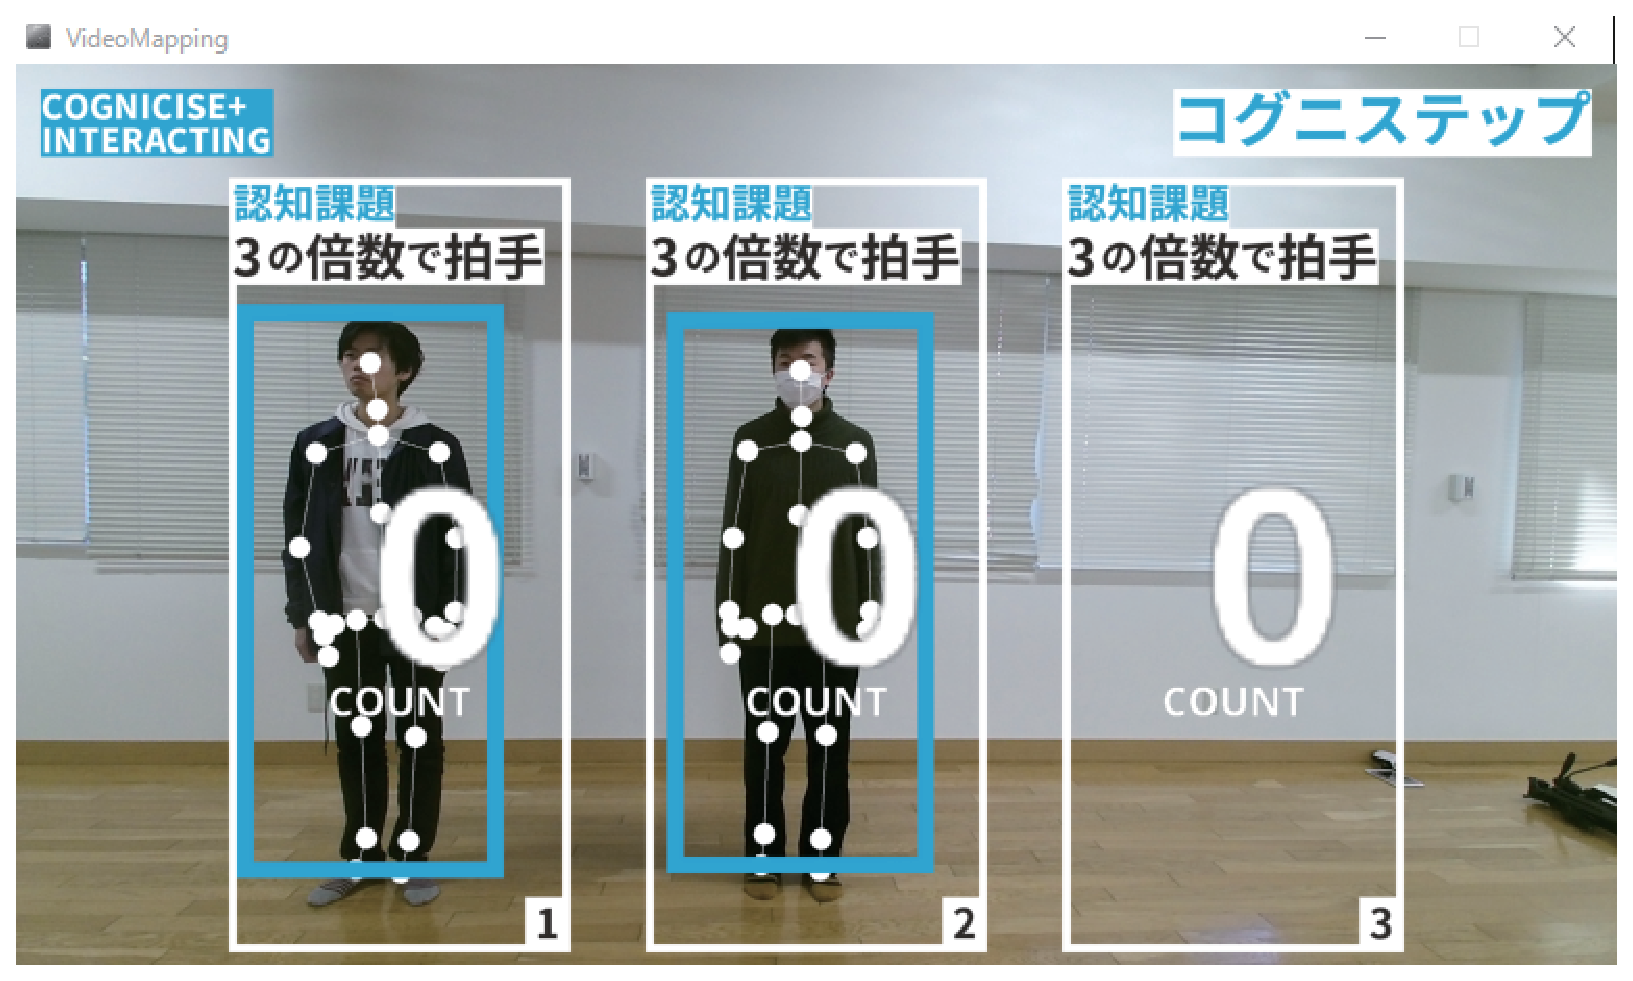
\includegraphics[width=.47\textwidth]{vm_init.eps}
\caption{プロジェクタ投影面}
\label{fig:vm_init}
\end{center}
\end{figure}

\begin{figure}[t]
\begin{center}
\includegraphics[width=.47\textwidth]{db_user_info.eps}
\caption{蓄積した認知課題の正答率の確認画面}
\label{fig:db_user_info}
\end{center}
\end{figure}

\begin{figure}[t]
\begin{center}
\includegraphics[width=.47\textwidth]{db_set_cognition.eps}
\caption{認知課題の負荷の調整画面}
\label{fig:db_init}
\end{center}
\end{figure}

\begin{figure}[t]
\begin{center}
\includegraphics[width=.4\textwidth]{use_system.eps}
\caption{実験の様子}
\label{fig:db_init}
\end{center}
\end{figure}

%--------------------------------------------
\section{実験と考察}
・認知課題の正誤判定の精度評価と考察

・提案システムを使用したコグニサイズの評価と考察

・提案システムに対する印象評価と考察


%--------------------------------------------
\section{まとめ}


%--------------------------------------------

\begin{thebibliography}{9}

%\bibitem{認知症とは}
%日本神経学会: ``認知症疾患治療ガイドライン2010''
\bibitem{認知症予防マニュアル}
国立長寿医療研究センター:``認知症予防マニュアル''
\bibitem{運動}
島田裕介: ``認知症予防を目的とした運動の効果''
\bibitem{コグニサイズとは}
国立長寿医療研究センター: ``コグニサイズとは?''
\bibitem{運動教室}
滝本幸治: ``地域に根ざした高齢者運動教室の効果検証''

\end{thebibliography}
\end{document}

%%% Local Variables: 
%%% mode: japanese-latex
%%% TeX-master: t
%%% End: 
